\documentclass[11pt]{amsart}
\usepackage{geometry}                % See geometry.pdf to learn the layout options. There are lots.
\geometry{letterpaper}                   % ... or a4paper or a5paper or ... 
%\geometry{landscape}                % Activate for for rotated page geometry
%\usepackage[parfill]{parskip}    % Activate to begin paragraphs with an empty line rather than an indent
\usepackage{graphicx}
\usepackage{amssymb}
\usepackage{epstopdf}
\DeclareGraphicsRule{.tif}{png}{.png}{`convert #1 `dirname #1`/`basename #1 .tif`.png}

\title{RGB zu Grayscale, Histogramm, Helligkeit}
\author{Andrey Borisov\\ Matrikel Nr.: 563858 \\ Andrey.Borisov@Student.HTW-Berlin.de}
%\date{}          
\usepackage{listings}
\usepackage{xcolor}
\usepackage[skins,listings,breakable]{tcolorbox}

                             % Activate to display a given date or no date
\renewcommand{\figurename}{Abb.}


\usepackage{footnote}
\makesavenoteenv{tabular}
\makesavenoteenv{table}
\usepackage{scrextend}


\begin{document}


\begin{titlepage}
\pagebreak
\hspace{0pt}
\vfill

\begin{center}

\fontsize{14}{17}\selectfont
\textit{Aufgabe 4}\\
\maketitle


\normalsize
\vspace{0.3cm}



\vspace{2cm}



%\textbf{H. Rakemann, 563176\\ N. Parschew, 563436 \\ R. Hänsch, 549390\\ A. Borisov, 563858}


\vspace{0.3cm}

\textit{HTW Berlin}

\vspace{0.1cm}

\textit{Programmierkonzepte und Algorithmen} \\
\vspace{0.3cm}
\textit{Prof. Dr. Nikita Kovalenko}



\end{center}

\vfill
\hspace{0pt}


\begin{figure}[htb]
 \raggedleft
 
\includegraphics[scale=0.4]{images/htwLogo.jpg}
\end{figure}
\vspace{-1cm}
\pagebreak
\end{titlepage}

\newpage

\tableofcontents
\newpage

























%\subsection{}

\section{Aufgabenstellung}
Das Ziel der gegebenen Aufgabe besteht darin, eine Anwendung zu entwickeln, die Bilder als Input bekommt, dann bestimmte Operationen mit diesen Bildern durchführt und anschließend die Ergebnisse anzeigt. Folgende Funktionalitäten müssen dabei umgesetzt werden:
\begin{itemize}
\item \textbf{RGB zu Grayscale:} Das Input-Bild muss von der Anwendung so transformiert werden, dass man ein Schwarzweiß-Bild als Output bekommt.
\item \textbf{Helligkeit:} Die Helligkeit des Input-Bildes muss um einen bestimmten Wert erhöht werden.
\item \textbf{Histogramm:} Die Anwendung sollte ein Histogramm des Input-Bildes erzeugen können und dieses anzeigen.
\end{itemize}

Eine weitere Anforderung besteht darin, die Anwendung so zu implementieren, dass alle Berechnungen parallel in mehreren Threads ausgeführt werden. Die implementierte Anwendung sollte in der Dokumentation beschrieben werden, wobei man insbesondere auf den Zusammenhang zwischen der Parallelisierung und der Ausführungsgeschwindigkeit eingehen muss. Außerdem muss die Ausführungsgeschwindigkeit von ähnlichen Anwendungen oder Libraries mit der Ausführungszeit der erstellten Anwendung für dieselben Operationen vergleichen.



\newpage
\section{Beschreibung der Lösung}

Für die Entwicklung der vorliegenden Anwendung wurde die Programmiersprache C++ benutzt. Um bestimmte Operationen an Bildern durchführen zu können, müssen diese Bilder vom Programm zuerst geladen werden, was mit der OpenCV-Bibliothek gemacht wird. Die Ausführung der implementierten Funktionalitäten wurde dabei mithilfe von OpenMP parallelisiert. Die umgewandelten Bilder und das Histogramm sollten dem Benutzer außerdem angezeigt werden, wofür ebenfalls die OpenCV Bibliothek benutzt wurde. Da das primäre Ziel der Parallelisierung die Verbesserung der Ausführungsgeschwindigkeit ist, wurde außerdem entschieden bestimmte Teile des Programms in Assembler zu implementieren, wodurch die Ausführung noch effizienter werden könnte\footnote{Ob das tatsächlich der Fall ist wird im Kapitel \ref{asmVSc++} untersucht}.

Nachfolgend werden die implementierten Funktionalitäten detailliert beschrieben.

\subsection{Bildtransformation-Funktionalitäten}\label{sec:picTransform}
Beide Bildtransformationen (Änderung der Helligkeit und RGB zu Grayscale) können sehr gut parallelisiert werden und zwar weil die einzelnen Threads nicht auf das Ergebnis anderer Threads warten müssen, da die einzelnen Pixel unabhängig von einander verarbeitet werden können. Das heißt insbesondere, dass die einzelnen Threads weder synchronisiert werden müssen, noch besitzen sie gemeinsame Variablen. Bei der Implementierung von den gegebenen Bildtransformationen können daher die einfachen for-Schleifen eingesetzt werden, deren Ausführung durch OpenMP parallelisiert werden kann: die erste Schleife wählt die Reihe und die zweite die Spalte des Pixels. Bei beiden Bildtransformationsoperationen wurde die äußere Schleife parallelisiert, da das in diesem Fall die effizienteste Methode ist, was im Abschnitt \ref{wahlParallel} gezeigt wird.

 
 

 
% b=b/14
 %g=g/1.39
 %r=r/4.55
 
 %183
 %127+63=190
 
 
\subsubsection{RGB zu Grayscale}\label{sec:gray}
Um ein RGB Bild in ein Grayscale-Bild umzuwandeln, müssen zuerst alle Werte des RGB Pixels zu einem Wert zusammengeführt werden. Danach wird dieser Wert jedem Kanal des RGB-Pixels zugewiesen, wodurch der Pixel einen bestimmten Grauton zugewiesen bekommt. Der Grauwert des Pixels kann zum Beispiel mit der folgenden Formel berechnet werden: 

 \begin{equation}\label{gray1}
 	gray = 0.21*r + 0.72*g + 0.07*b
\end{equation}

Wenn man jedoch bedenkt, dass die Pixel-Werte durch ganze Zahlen (Werte zwischen 0 und 255) und nicht durch Float-Zahlen dargestellt werden, kann man die Multiplikation mit Float-Zahlen durch die Division mit ganzen Zahlen ersetzen. Das würde zur folgenden Gleichung führen:

 \begin{equation}\label{gray2}
 	gray = r/4 + (g/2 + g/4) + b/14
\end{equation}

Die RGB zu Grayscale Funktionalität wurde in Assembler implementiert: deshalb sollte man bei der Division die Zweierpotenzen benutzen, da dies besonders effizient ist. Somit ergibt sich die Folgende Gleichung:

 \begin{equation}\label{gray3}
 	gray = r/4 + (g/2 + g/4) + b/16
\end{equation}

Der Quellcode der RGB zu Grayscale Funktionalität ist im Listing 1 zu sehen. Die Umwandlung wurde durch OpenMP parallelisiert und zwar nur die äußere Schleife. Als erstes wird der RGB-Wert geladen: anstatt die Werte der RGB-Kanäle einzeln aus dem Speicher zu laden, wird der ganze RGB in den \textit{EAX} Register mit nur einem Speicherzugriff geladen. Danach werden an \textit{EAX} Operationen durchgeführt, die zu denen aus der Gleichung \ref{gray3} äquivalent sind. Anschließend wird der berechnete Grayscale-Wert in den Speicher des entsprechenden Pixels geschrieben. Ein Beispiel für die Umwandlung mit dieser Implementierung ist auf der Abb. \ref{fig:grayscaleExample} zu sehen.



  \begin{tcblisting}{breakable,listing only,
  listing options={language=c,aboveskip=0pt,belowskip=0pt},
  size=fbox,boxrule=0pt,frame hidden,arc=0pt,colback=lightgray,title=Listing 1: RGB to Grayscale}
#pragma omp parallel for
     for (int i = 0; i < rows; ++i) {
         for (int j = 0; j < cols; ++j) {
             uchar* pixel = ptr + channels * (i * cols + j);
             __asm {
                     mov rcx, pixel    //rcx = pixel
                     mov eax, [rcx]    //eax=*rcx   -> eax=bgr

                     shr al, 4    //al=al/16
                     shr ah, 1    //ah=ah/2
                     add al, ah   //al=al+ah	    
                     shr ah, 1    //ah=ah/2
                     add ah, al  //ah=ah+al

                     shr eax, 8    //shift the r-Value into ah
                     shr ah, 2    //ah=ah/2
                     add al, ah  //al=al+ah    	
                     jnc label    //check if value <= 255 
                     mov al, 255

             label:
             	    //*pixel = rgb(al,al,al)
                     mov [rcx], al  
                     mov [rcx+1], al
                     mov [rcx+2], al
             }
         }
     }
\end{tcblisting}
\newpage
\begin{figure}[thb!]
\begin{minipage}{8cm}
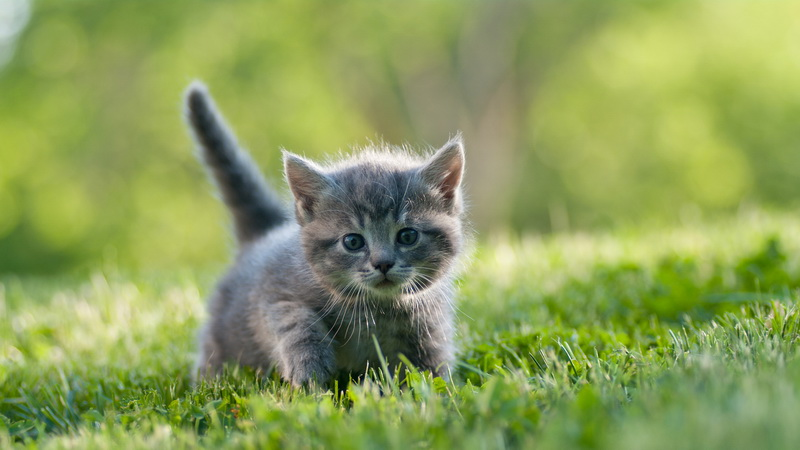
\includegraphics[width=8cm]{images/original.jpg}
\end{minipage}
\qquad
\begin{minipage}{8cm}
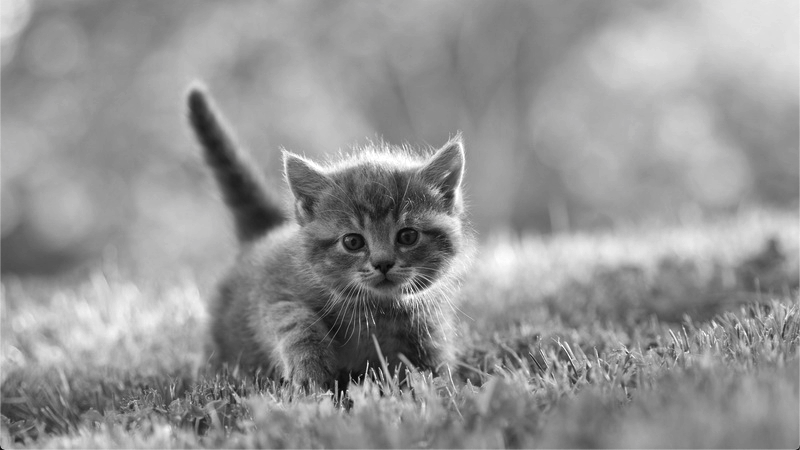
\includegraphics[width=8cm]{images/myRGB.png}
\end{minipage}
\caption{Umwandlung: RGB zu Grayscale}
\label{fig:grayscaleExample}
\end{figure}

\subsubsection{Helligkeit}
Die Helligkeit eines Bildes kann verändert werden, indem man eine konstante Zahl mit jedem Kanal von jedem Pixel summiert. Dies kann mit der folgenden Gleichung beschrieben werden:

 \begin{equation}\label{helligkeit}
 	pixel = rgb(r+\alpha, g+\alpha, b+\alpha)
\end{equation}

%Auch hier macht es wenig Sinn Float-werte zu verwenden, da die Kanäle der Pixel durch ganze Zahlen dargestellt werden.

Auch bei dieser Operation ist es sinnvoller mit ganzen Zahlen zu arbeiten, da die Kanäle der Pixel durch ganze Zahlen dargestellt werden. Beim Summieren muss man jedoch darauf achten, dass die resultierenden Werte den Wert 255 nicht übersteigen. Im Listing 2 sieht man wie das Anpassen der Helligkeit implementiert wurde. Bei der Implementierung wurden SIMD-Operationen\footnote{Single Instruction, Multiple Data} des x86-Assemblers verwendet: zuerst werden die Daten eines Pixels in den mm1-Register geladen und dann wird ein Array bestehend aus den Helligkeitswerten, die dazuaddiert werden sollten, in den Register mm0 geladen. Danach werden beide Register mit nur einer Operation paddusb\footnote{Eine SIMD Operation: Add Packed Unsigned Integers with Unsigned Saturation} summiert. Das Ergebnis der Addition wird dann in den Speicher des Pixels geschrieben. Auf der Abb. \ref{fig:hellExample} sieht man ein Beispiel für die Umwandlung eines Bildes mit dieser Funktionalität.


  \begin{tcblisting}{breakable,listing only,
  listing options={language=c,aboveskip=0pt,belowskip=0pt},
  size=fbox,boxrule=0pt,frame hidden,arc=0pt,colback=lightgray,title=Listing 2: Helligkeit}
uchar brightnessArr[4] = {brightness, brightness, brightness, 0};
#pragma omp parallel for
     for (int i = 0; i < rows; ++i) {
         for (int j = 0; j < cols; ++j) {
             uchar* pixel = ptr + channels * (i * cols + j);
             __asm {
                     mov rcx, pixel
                     movd mm1, [rcx]
                     movd mm0, brightnessArr
                     paddusb mm1, mm0
                     movd [rcx], mm1
             }
        }
     }
\end{tcblisting}

\newpage
\begin{figure}[thb!]
\begin{minipage}{8cm}
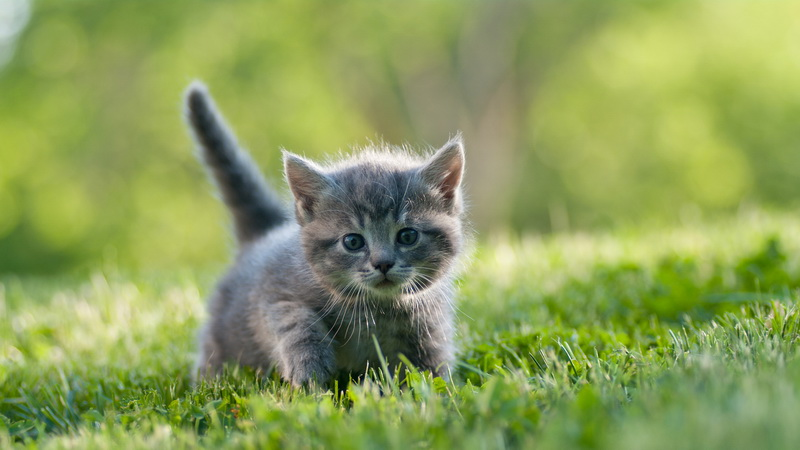
\includegraphics[width=8cm]{images/original.jpg}
\end{minipage}
\qquad
\begin{minipage}{8cm}
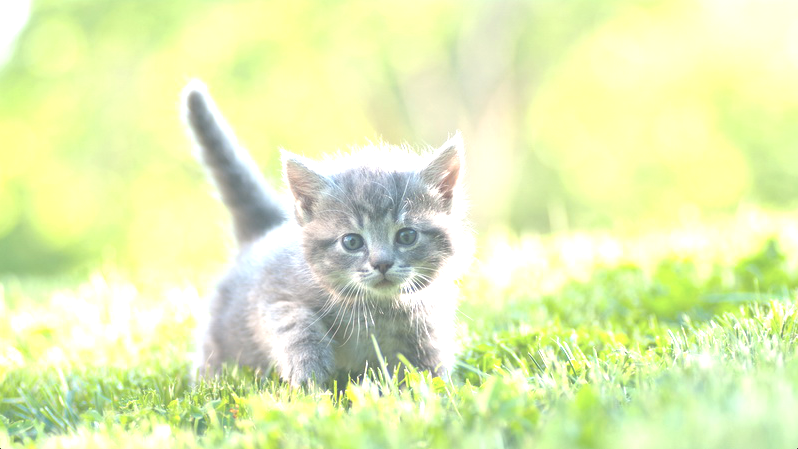
\includegraphics[width=8cm]{images/myHelligkeit.png}
\end{minipage}
\caption{Umwandlung: Helligkeit + 100}
\label{fig:hellExample}
\end{figure}



\subsection{Histogramm}
Bei dem der Erstellung des Histogramms eines Bildes zählt man die Kanäle aller Pixel, die denselben Wert haben und erstellt dann eine Abbildung, die die ermittelten Werte darstellt. Da die Kanäle der Pixel den Wertebereich 0-255 haben, gibt es dabei 256 Zähler für jeden Farbkanal des Pixels. Das Erstellen des Histogramms kann in drei Schritte aufgeteilt werden:

\begin{enumerate}
\item Werte der Farbkanäle der Pixel werden gezählt.
\item Der höchste Wert unter allen Zählern wird bestimmt (Dieser Wert wird beim Zeichnen des Histogramms benötigt, damit das Histogramm richtig skaliert wird).
\item Das Histogramm wird gezeichnet.
\end{enumerate}

Bei dem ersten Schritt braucht man einen Zähler-Array für jedes Farbkanal. Es ist klar, dass im Falle der Parallelisierung des ersten Schrittes mit \textit{"\#pragma omp parallel for"}, es zu Race-Conditions kommen wird, da unterschiedliche Threads gleichzeitig auf den Wert eines bestimmten Zählers zugreifen und diesen manipulieren könnten. Damit keine Race-Conditions entstehen können wird stattdessen \textit{"\#pragma omp parallel for reduction"} für die Parallelisierung benutzt. Im Listing 3 kann man sehen, dass die dabei verwendete Reduktionsoperation '+' ist, wobei diese auf die drei Zähler-Arrays angewendet wird. An dieser Stelle könnte man alternativ die Zähler-Arrays bei der parallelisierten For-Schleife als 'shared' festlegen, jedoch wurde festgestellt, dass die bereits beschriebene 'reduction'-Methode bei der Ausführung effizienter ist\footnote{Wird im Abschnitt \ref{sec:evalHist} gezeigt}.

  \begin{tcblisting}{breakable,listing only,
  listing options={language=c,aboveskip=0pt,belowskip=0pt},
  size=fbox,boxrule=0pt,frame hidden,arc=0pt,colback=lightgray,title=Listing 3: Schritt 1}
 #pragma omp parallel for reduction(+ \
                                    : histogramDataR,\ 
                                      histogramDataG,\ 
                                      histogramDataB)
         for (int i = 0; i < rows; ++i) {
             for (int j = 0; j < cols; ++j) {
                 uchar* pixel = ptrImg + channels*( i*cols + j);
                 histogramDataB[pixel[0]] += 1;
                 histogramDataG[pixel[1]] += 1;
                 histogramDataR[pixel[2]] += 1;
             }
         }
\end{tcblisting}

Im zweiten Schritt muss der höchste Wert, der in einem der Zähler-Arrays ist, ermittelt werden. Die Implementierung des zweiten Schritts ist im Listing 4 zu sehen: bei diesem Schritt wurde ebenfalls die 'reduction'-Methode eingesetzt, allerdings mit der 'max' Operation. Der ermittelte Maximal-Wert wird in der \textit{highestCounter}-Variable gespeichert.

  \begin{tcblisting}{breakable,listing only,
  listing options={language=c,aboveskip=0pt,belowskip=0pt},
  size=fbox,boxrule=0pt,frame hidden,arc=0pt,colback=lightgray,title=Listing 4: Schritt 2}
        int highestCounter = 0;
 #pragma omp parallel for reduction(max : highestCounter)
        for (int i = 0; i < 256; ++i) {
             if (histogramDataB[i] > highestCounter) {
                 highestCounter = histogramDataB[i];
             }
             if (histogramDataG[i] > highestCounter) {
                 highestCounter = histogramDataG[i];
             }
            if (histogramDataR[i] > highestCounter) {
                 highestCounter = histogramDataR[i];
             }
         }
   \end{tcblisting}     
   
   Im dritten Schritt wird das Histogramm erstellt. Wie das Histogramm erstellt wird, kann man im Listing 5 sehen. Die Ausführung von diesem Schritt wurde nur durch \textit{\#pragma omp parallel for} parallelisiert. Die Größe des Histogramms kann durch den Parameter \textit{'scale'} festgelegt werden. Ein erstelltes Beispiel-Histogramm ist auf der Abb. \ref{fig:histExample} zu sehen: blaue Farbe gehört zum b-Kanal, grüne Farbe zum g-Kanal und rote zum r-Kanal.
 
   \begin{tcblisting}{breakable,listing only,
  listing options={language=c,aboveskip=0pt,belowskip=0pt},
  size=fbox,boxrule=0pt,frame hidden,arc=0pt,colback=lightgray,title=Listing 5: Schritt 3}      
#pragma omp parallel for
       for (int i = 0; i < 256 * scale; i += 1 * scale) {
           float r = histogramDataR[i / scale];
           float g = histogramDataG[i / scale];
           float b = histogramDataB[i / scale]         
           for (int j = 0; j < rows; ++j) {
               uchar* pixel = ptrHist+channels*(j*cols + i);
               float rowTemp = (float)j / histMatrix.rows;
               if (r / highestCounter > rowTemp) {
                   pixel[2] = 255;
               }  
               if (g / highestCounter > rowTemp) {
                   pixel[1] = 255;
               }
               if (b / highestCounter > rowTemp) {
                   pixel[0] = 255;
               }
           }
       }
\end{tcblisting}


\newpage
\begin{figure}[thb!]
\begin{minipage}{8cm}
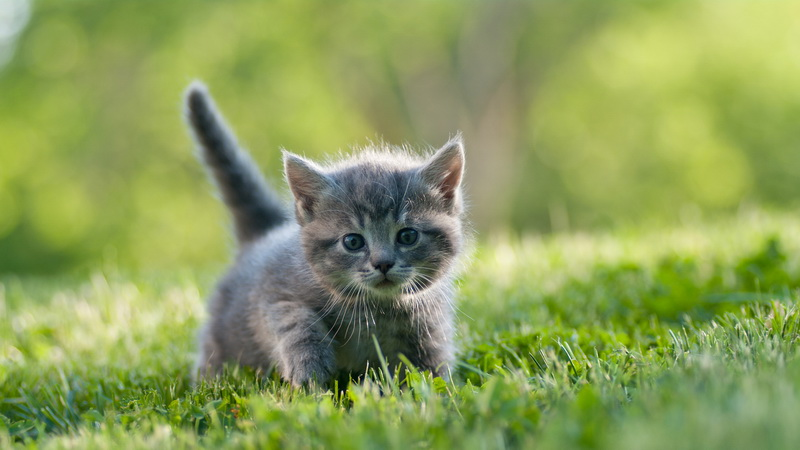
\includegraphics[width=8cm]{images/original.jpg}
\end{minipage}
\qquad
\begin{minipage}{8cm}
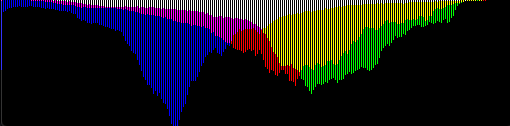
\includegraphics[width=8cm]{images/myHisto.png}
\end{minipage}
\caption{Erstelltes Histogramm}
\label{fig:histExample}
\end{figure}


\subsection{Konsolen-User-Interface}

Das implementierte Anwendung lässt sich durch Konsole-Argumente steuern. Folgende Argumente sind zulässig:


\begin{tabular}[h]{|l|l|}
\hline
\textbf{Argument} & \textbf{Beschreibung}  \\
\hline
-p [path] & Legt den Pfad zum Bild fest, das untersucht werden soll. \\
\hline
-g & Aktiviert die Umwandlung von RGB zu Grayscale. \\
\hline
-s & Wenn das Original-Bild auch angezeigt werden soll. \\
\hline
-b [brightness] & Addiert den Wert \textit{brightness}(integer) zur Helligkeit.\\
\hline
-t [numOfThreads] & Zum ändern der Anzahl an aktiven Threads.\\
\hline
-pn& Dadurch wird nur die Ausführungszeit ausgegeben\footnote{Diese Option ist für das automatisierte Testing notwendig\label{refnote}}.\\
\hline
-c& Das Problem wird automatisch geschlossen nach dem die Ausführung fertig ist\footref{refnote}.\\
\hline
-h [scale]& Legt fest ob ein Histogramm erzeugt werden soll und falls ja wie groß(=scale).\\
\hline
-cpp & Sorgt dafür, dass nur reiner C++ Code (=ohne Assembler) ausgeführt wird.\\
\hline
\end{tabular}










\newpage
\section{Evaluierung}
In diesem Kapitel wird die erstellte Anwendung detailliert evaluiert und untersucht. Bei jedem durchgeführten Test wurde die getestete Funktionalität 50 mal ausgeführt, sodass am Ende ein arithmetisches Mittel von den ermittelten Ausführungszeiten errechnet werden konnte. Die Tests wurden auf einem Rechner mit einem Intel i5 Prozessor der 10 Generation unter macOS durchgeführt.








\subsection{Wahl der Parallelisierungsart} \label{wahlParallel}
OpenMP bietet mehrere unterschiedliche Werkzeuge an, mit denen man die Ausführung von bestimmten Vorgängen parallelisieren kann. Es ist dabei wichtig, dass man die Werkzeuge wählt, die für eine bestimmte Aufgabe geeignet sind.

\subsubsection{Parallelisierung von Bildtransformation-Operationen}
Bei den beiden Bildtransformation-Operationen (Grayscale und Helligkeit) werden zwei Schleifen gebraucht: eine um die Reihe des Pixel auszuwählen und eine für die Wahl der Spalte des Pixels. Es gibt dabei mehrere Möglichkeiten die einzelnen Pixel mit OpenMP parallel zu verarbeiten. Folgende Varianten wurden bei der Wahl der optimalen Lösung untersucht:
 

  
  \begin{tcblisting}{breakable,listing only,
  listing options={language=c,aboveskip=0pt,belowskip=0pt},
  size=fbox,boxrule=0pt,frame hidden,arc=0pt,colback=lightgray,title=Variante 1}
#pragma omp parallel for
for (int i = 0; i < rows; ++i) {
    for (int j = 0; j < cols; ++j) {
        ...
    }
}
\end{tcblisting}



  \begin{tcblisting}{breakable,listing only,
  listing options={language=c,aboveskip=0pt,belowskip=0pt},
  size=fbox,boxrule=0pt,frame hidden,arc=0pt,colback=lightgray,title=Variante 2}
for (int i = 0; i < rows; ++i) {
#pragma omp parallel for
    for (int j = 0; j < cols; ++j) {
        ...
    }
}
\end{tcblisting}

  \begin{tcblisting}{breakable,listing only,
  listing options={language=c,aboveskip=0pt,belowskip=0pt},
  size=fbox,boxrule=0pt,frame hidden,arc=0pt,colback=lightgray,title=Variante 3}
#pragma omp parallel for collapse(2)
for (int i = 0; i < rows; ++i) {
    for (int j = 0; j < cols; ++j) {
        ...
    }
}
\end{tcblisting}

Bei der ersten Variante wird die äußere Schleife parallelisiert. Bei der zweiten wird dagegen die innere Schleife parallelisiert. Die dritte Variante wandelt beide Schleifen durch "collapse(2)" in eine Schleife um, sodass aus allen Iterationen beider Schleifen ein großer Iterationsraum gebildet wird, der dann unter den Threads des Programms aufgeteilt werden kann.

Alle drei Varianten wurden untersucht: die Varianten wurden anhand der RGB zu Grayscale Umwandlung getestet, wobei jede Variante 50 mal ausgeführt wurde und ein arithmetisches Mittel zu jeder Variante berechnet wurde. Die Ergebnisse sind auf der Abb. \ref{fig:testFor} zu sehen. Man sieht, dass die erste Variante eine viel bessere Ausführungszeit hat, weshalb diese Variante bei der Implementierung von den Bildtransformation-Funktionalitäten gewählt wurde. Dass die Ausführungszeiten der vorgestellten Parallelisierungs-Varianten so unterschiedlich sind hängt womöglich damit zusammen, dass die Caching-Mechanismen des Prozessors mit einigen Varianten besser kompatibel sind als mit den anderen.

 \begin{figure}
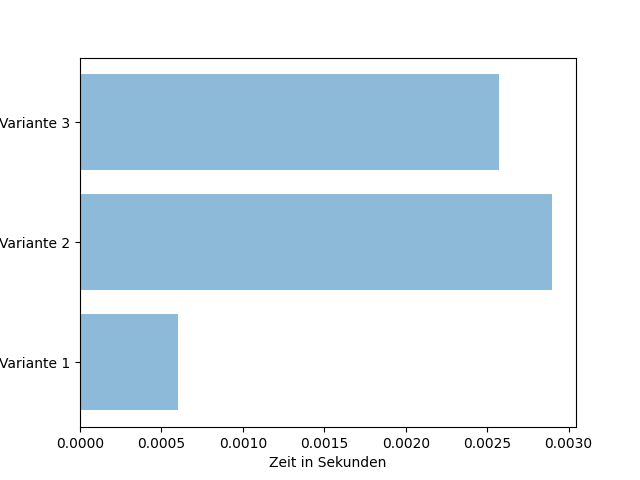
\includegraphics[scale=0.6]{images/testFor.png}
\caption{Vergleich von Varianten der Parallelisierung}
\label{fig:testFor}
\end{figure}


\subsubsection{Parallelisierung der Histogramm-Erstellung} \label{sec:evalHist}
Bei der Erstellung des Histogramms ist es so, dass die Threads nicht unabhängig voneinander sind, wie das bei den Bildtransformation-Operationen der Fall war. Aber auch für dieses Problem, bietet OpenMP mehrere Lösungswege an. Es wurden zwei mögliche Lösungen gewählt und untersucht:

\begin{itemize}
\item \textbf{Shared:} wie der Name bereits verrät, werden bei dieser Variante bestimmte Variablen unter den Threads geteilt, sodass es keine Race-Conditions entstehen können. Wird mit der Pragma-Anweisung \textit{"\#pragma omp parallel for shared(\%varName\%)"} aktiviert.
\item \textbf{Reduction:} bei dieser Variante werden die Threads zunächst unabhängig ausgeführt, ohne dass die Variablen unter den Threads synchronisiert werden und am Ende werden die Teilergebnisse der Threads gesammelt und zu einem Ergebnis kombiniert. Wird mit der Pragma-Anweisung \textit{"\#pragma omp parallel for reduction(\%operation\% : \%varName\%)"} aktiviert.
\end{itemize}

 \begin{figure}
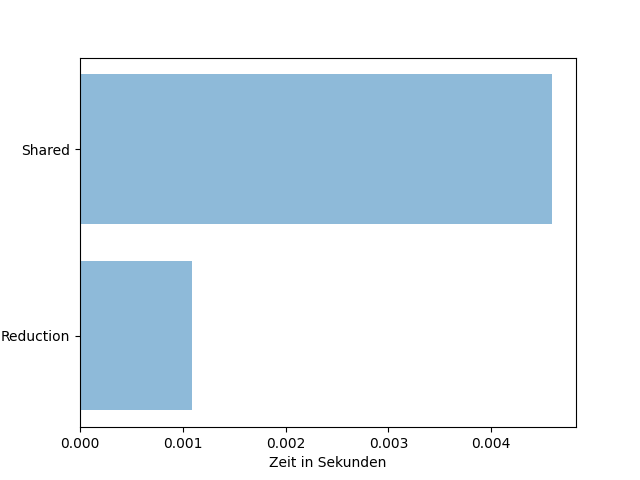
\includegraphics[scale=0.6]{images/sharedVSreduction.png}
\caption{Vergleich von \textit{shared} und \textit{reduction}}
\label{fig:sharedVSreduction}
\end{figure}

Beide Varianten wurden getestet und die dabei ermittelten Ausführungszeiten kann man auf der Abb. \ref{fig:sharedVSreduction} sehen. Man sieht, dass die Reduction-Variante mindestens vier Mal so schnell ist wie die Shared-Variante, weshalb diese Variante bei der Implementierung gewählt wurde. Dass die Shared-Variante so viel langsamer ist liegt daran, dass die Variable, die von mehreren Threads geteilt wird, unter allen Threads synchronisiert werden muss, weshalb die Ausführung sehr verlangsamt wird. Bei der Reduction-Variante werden die Teilergebnisse der Threads dagegen erst nach dem Beenden der Schleife kombiniert, sodass bei der Ausführung der Schleife nichts synchronisiert werden muss und die Ausführungszeit dadurch viel besser ist. 


%reduction= 0.001090 s 
%shared= 0.004594 s




 \begin{figure}[thb!]
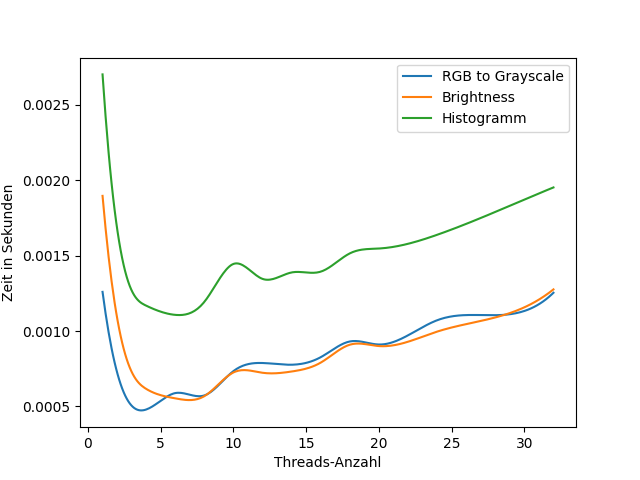
\includegraphics[scale=0.6]{images/threadsNumber.png}
\caption{Zusammenhang der Threads-Anzahl mit der Ausführungszeit}
\label{fig:threadsNumber}
\end{figure}

\subsubsection{Optimale Threadsanzahl}
Bei der parallelen Abarbeitung einer Aufgabe kann man die Anzahl an Threads, die für das Abarbeiten dieser Aufgabe zuständig sind, wählen. Es ist dabei klar, dass von der Anzahl der Threads die Ausführungszeit des Programms abhängig ist. Es ist jedoch so, dass es nicht immer der Fall ist, dass mit einer größeren Threads-Anzahl die bessere Ausführungszeit erzielt wird: wenn die Threads-Anzahl zu groß wird kann es sogar negative Auswirkungen auf die Ausführungszeit haben. Wie viele Threads zu einer optimalen Ausführungszeit führen könnte, wird maßgeblich von den Eigenschaften des Prozessors, wie die Anzahl an Cores oder Threads beeinflusst. Meistens lohnt es sich die Anzahl an Threads auf eine Zahl zu setzen, die größer ist als  die Anzahl an Cores des Prozessors, da durch die Cores-Anzahl die Anzahl an parallel ausführbaren Threads festgelegt wird. Es muss jedoch nicht unbedingt der Fall sein, dass die Anzahl an Cores tatsächlich die optimale Anzahl an Threads für ein Programm ist, da Prozessoren heutzutage sehr komplex sind und außerdem von anderen Komponenten (wie z.B. Arbeitsspeicher und Festplatte) abhängen.

Der Zusammenhang zwischen der Ausführungszeit der implementierten Anwendung und der Anzahl an Threads wurde untersucht. Bei der Ausführung von Tests wurde ein Rechner mit dem i5 Prozessor der zehnten Generation verwendet (4 Cores und 8 Threads), wobei alle drei Funktionalitäten separat voneinander untersucht wurden (RGB to Grayscale, Helligkeit-Änderung und Histogramm). Die Ergebnisse dieser Untersuchung sind auf der Abb. \ref{fig:threadsNumber} zu sehen. Man sieht, dass alle drei Kurven recht ähnlich zueinander sind, jedoch trotzdem gewisse Unterschiede aufweisen. Die optimale Anzahl an Threads ist bei der \textit{RGB to Grayscale} Operation liegt bei 4 Threads, was mit der Anzahl an Cores des gegebenen Prozessors übereinstimmt. Dagegen liegt die optimale Anzahl von Threads bei der \textit{Helligkeit-} und \textit{Histogramm}-Operation interessanterweise bei 6 Threads, was zeigt, dass die optimale Threads-Anzahl nicht immer mit der Anzahl an Cores des Prozessors übereinstimmen muss.

Es ist außerdem wichtig zu untersuchen welche Auswirkung die Parallelisierung an sich auf das Programm hat: bei Grayscale ist die Ausführung mit der optimalen Anzahl an Threads 162\% besser als die Ausführung mit einem Thread und analog beträgt die Verbesserung bei der Brightness Operation 242\% und beim Histogramm 144\%.






%histogram:
%1 0.0027015254
 %2 0.0016804414
 %4 0.00116811682
% 6 0.001107135
% 8 0.0011936620800000002
% 10 0.0014448643999999998
% 12 0.0013456873999999998
 %14 0.0013884396000000002
 %16 0.0013937186
 %18 0.0015148829999999996
 %20 0.0015470647999999995
%24 0.0016378978000000002
% 28 0.001789608
 %32 0.0019520376

%gray:
%1 thread: 0.0012596
%2 thread: 0.0007259
%4 thread: 0.0004797
%6 thread: 0.0005886
%8 thread:  0.0005730
%10 thread: 0.0007344
%12 thread: 0.0007880
%14 thread: 0.00077658
%16 thread: 0.00082656
%18 thread: 0.0009307813
%20 thread: 0.000910601
%24 thread: 0.0010714
%28 thread: 0.0011050
%32 thread: 0.0012538

%brightness:
%1 thread: 0.0018961
%2 thread: 0.0010882
%4 thread: 0.0006163
%6 thread: 0.0005535
%8 thread:  0.000568208
%10 thread: 0.00072548
%12 thread: 0.00072319
%14 thread: 0.000731563
%16 thread: 0.00079058
%18 thread: 0.000909390
%20 thread: 0.0009003639
%24 thread:  0.00099605
%28 thread: 0.00109001
%32 thread: 0.0012760497

 %mein processor hat 12 threads und 6 cores anscheinend
 
 


 \begin{figure}[thb!]
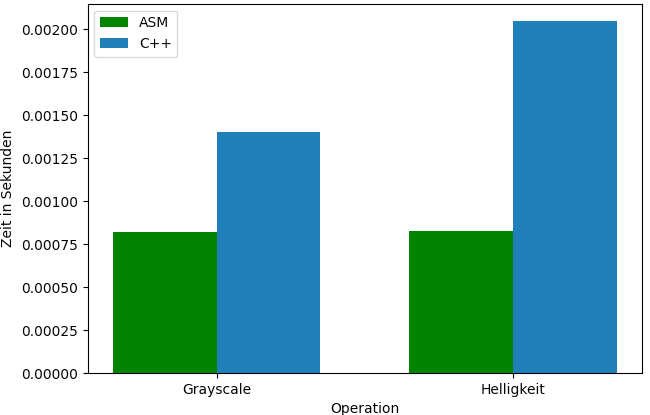
\includegraphics[scale=0.5]{images/asmVScpp.png}
\caption{Vergleich der Ausführungszeit von C++ mit Assembler}
\label{fig:asmVScpp}
\end{figure}

\subsection{Vergleich mit alternativen Implementierungen}


\subsubsection{Vergleich von Assembler mit C++} \label{asmVSc++}
Bei der Implementierung der beiden Bildtransformation-Operationen wurden bestimmte Teile des Programms in Assembler implementiert. Es wäre interessant zu untersuchen ob die Assembler-Implementierung tatsächlich besser als eine C++ Implementierung ist, denn die modernen Kompilierer besitzen effektive Optimierungsmechanismen, sodass eine Assembler-Implementierung nicht immer effizienter ist als das vom Kompilierer generierte Programm.

Um zu untersuchen, ob die in Assembler implementierte Teile der Anwendung effizienter sind als reiner C++ Code, wurden die entsprechenden Teile der Anwendung in C++ implementiert, sodass man beide Varianten verlgleichen kann. Auf der Abb. \ref{fig:asmVScpp} sieht man die Ergebnisse: man sieht, dass die erstellte Assembler-Implementierung deutlich bessere Ausführungszeit hat als das äquivalente C++ Programm.



%brightness c++:  0.002048126
%brightness asm:   0.00082451338
 
%grayscale c++:  0.00140189582
%grayscale asm:  0.00082184782

 \begin{figure}
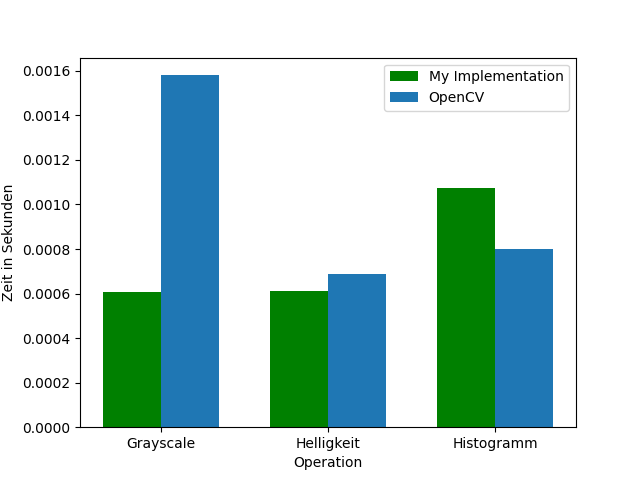
\includegraphics[scale=0.65]{images/openCVvsMy.png}
\caption{Vergleich der Ausführungszeit von OpenCV und der implementierten Anwendung}
\label{fig:opencvVSmy}
\end{figure}

\subsubsection{Vergleich mit OpenCV}
%--opencv:
%gray:0.0015803
%helligkeit: 0.000686330
%histogram:0.0007980

%--myImplementation:
%gray:0.00060810
%helligkeit: 0.00060926
%histogram: 0.00107450

Die Performance der Implementierten Anwendung kann außerdem mit anderen Implementierungen von ähnlichen Funktionalitäten verglichen werden. Mit der OpenCV Bibliothek lassen sich schnell Funktionalitäten erstellen, die zu den Funktionalitäten der implementierten Anwendung äquivalent sind. Die Ergebnisse des Vergleichs kann man auf der Abb. \ref{fig:opencvVSmy} sehen. Man sieht, dass die Grayscale- und die Helligkeit-Operation bei der implementierten Anwendung schneller als bei OpenCV ist, wobei insbesondere bei der Grayscale-Operation der unterschied recht groß ist (159\% schneller). Bei der Erstellung des Histogramms ist OpenCV allerdings schneller (34\% schneller), was vermutlich durch eine effizientere Implementierung zustande kommt.





\section{Zusammenfassung}


Im Rahmen dieser Arbeit wurde eine Anwendung entwickelt, die zwei Bildtransformation-Operationen (Grayscale und Helligkeit-Änderung) und eine Operation zur Bildanalyse (Histogramm) enthält. Die Ausführung der implementierten Funktionalitäten wurde dabei zwecks der schnelleren Ausführung mit OpenMP parallelisiert. Während der Implementierung wurden mehrere unterschiedliche Möglichkeiten der Parallelisierung in Betracht gezogen und analysiert, sodass man für die finale Implementierung die optimalere Methode nehmen konnte.

 Des Weiteren wurden einige Teile der Anwendung in Assembler implementiert, was ebenfalls zu einer Verbesserung der Ausführungsgeschwindigkeit geführt hat. Dass die implementierte Anwendung effizient ist, wurde auch durch den Vergleich der beschriebenen Anwendung mit der OpenCV Implementierung gezeigt: beide Bildtransformation Operationen waren effizienter als die OpenCV Implementierung und nur die Histogramm-Berechnung war etwas schlechter als die OpenCV Implementierung. 









\end{document}  